\clearpage
\setcounter{page}{1}
\maketitlesupplementary
\appendix

In this supplementary material, we provide additional details omitted from the main manuscript. Sec.~\ref{subsec:impl} describes the implementation details and the 3D tasks under evaluation. Sec.~\ref {subsec:eval_prot} outlines the experimental setup and the 3D semantic segmentation evaluation protocol on 3D Gaussian Splatting. Sec.~\ref{subsec:robust} further presents a robustness study, where we stress-test our method under corrupted SAM masks to assess performance degradation in noisy segmentation scenarios.  while Sec.~\ref{subsec:add_results} presents qualitative results, annotation analyses, and city-scale evaluations. Finally, Sec.~\ref{subsec:limt} discusses limitations and future directions. 

\section{Implementation Details}
\label{subsec:impl}

Our method operates in two stages. In the pre-training stage, we apply the ViT-H variant of SAM~\cite{kirillov2023sam} to segment each image. Multi-level language feature maps are then extracted with OpenCLIP ViT-B/16~\cite{radford2021clip}, from which we derive per-patch language embeddings. In parallel, we optimize the 3D Gaussian Splatting parameters~\cite{kerbl20233d} using the standard training pipeline with the \emph{gsplat} rasterizer~\cite{ye2025gsplat}, running 30k iterations. Unlike the original rasterizer, \emph{gsplat} natively supports rendering high-dimensional Gaussian attributes, which enables evaluation on 2D open-vocabulary tasks.

In the subsequent forward-rendering stage, we adopt the feature aggregation strategy of Occam’s LGS~\cite{cheng2024occam}. For each Gaussian within the view frustum, we compute its center-projected pixel location and extract the corresponding 2D language feature $f_i^s$. Simultaneously, we record its marginal contribution $w_i(r)$ as defined in Eq.~\eqref{eq:visibility_weights}, and retain the most visible Gaussians following the gating strategy in Sec.~\ref{sec:gating}. The selected Gaussians are then robustly aligned with multi-view features through our streaming aggregation in cosine space, described in Sec.~\ref{sec:median}.

This entire process completes within 10 seconds to one minute per scene (depending on scene scale) without memory overflow. All experiments are conducted on an NVIDIA RTX 4090 GPU.

\section{Evaluation Protocols}
\label{subsec:eval_prot}
We only compare results following the same evaluation protocol and re-evaluate those prior works that followed other protocols.

\textbf{Datasets}
We evaluate our method on two datasets: LERF-OVS~\cite{qin2024langsplat} and ScanNet~\cite{dai2017scannet}. LERF-OVS consists of four scenes (teatime, waldo\_kitchen, figurines, ramen), each annotated with pixel-wise semantic masks and paired with short text queries. In this dataset, we evaluate open-vocabulary object selection in both 2D and 3D settings. To further evaluate 3D semantic segmentation, we adopt a Gaussian-based evaluation protocol on ScanNet, a large-scale RGB-D dataset for indoor scene understanding. Each ScanNet sequence is reconstructed into a textured 3D mesh with globally aligned camera poses and semantic annotations. We select eight representative scenes covering diverse indoor environments, including living rooms, bathrooms, kitchens, bedrooms, and meeting rooms.

\textbf{2D and 3D Evaluation on the LERF-OVS Dataset.}
For the 2D evaluation, we follow the protocol of LERF~\cite{kerr2023lerf}: 512-dimensional feature maps are rendered, and a relevancy map is computed with respect to the CLIP-embedded text query. The relevancy map is then thresholded at 0.5 to obtain the predicted binary mask. For the 3D evaluation, we adopt the protocol of OpenGaussian~\cite{wu2024opengaussian}, where the relevancy score between each 3D Gaussian’s language embedding and the text query embedding is computed and thresholded at 0.6. The alpha values of the selected Gaussians are subsequently projected onto the image plane to generate the predicted mask. In both cases, the predicted masks are compared against the GT annotations of the LERF-OVS dataset.

\textbf{3D Semantic Segmentation on the ScanNet-v2 Dataset.}
Previous works on 3D semantic segmentation~\cite{wu2024opengaussian, li2024instancegaussian} typically freeze the input point cloud (derived from ground-truth annotations) during 3D Gaussian Splatting training to cope with the absence of GT labels as the point clouds evolve. However, this strategy degrades the 2D rendering quality of 3DGS. We instead propagate ground-truth (GT) labels from the annotated point cloud to the Gaussians, thereby obtaining pseudo-GT labels at each Gaussian’s 3D mean. Following OpenGaussian~\cite{wu2024opengaussian}, we evaluate on subsets of 19, 15, and 10 of the 40 most common classes. For each class, we encode the text label using CLIP~\cite{radford2021clip} to obtain a 512-dimensional embedding, and compute its cosine similarity with the registered language features of each Gaussian. Each Gaussian is then assigned to the class with the highest similarity score. Performance is measured in terms of mIoU and mAcc against the pseudo-GT Gaussian point cloud.


\noindent\textbf{Pseudo-Gaussian Labeling.}
% Inspired by Kim~\etal~\cite{drsplat25}, we instead first train 3D Gaussian Splatting without restrictions and subsequently propagate labels from the ground-truth point cloud to the optimized Gaussians, explicitly accounting for their scales and rotations. 
Given optimized Gaussians 
$\Theta=\{\theta_i\}_{i=1}^N$ 
with center $\mu_i$, scale $s_i=(s_{ix},s_{iy},s_{iz})$, rotation $R_i$ 
(hence $\Sigma_i = R_i \,\mathrm{diag}(s_i^2)\,R_i^\top$), and opacity $\alpha_i$, 
and a labeled point cloud $\{(p_k,s_{p_k})\}_{k=1}^Q$, 
we assign a semantic label to each Gaussian by respecting the \emph{true} 3DGS geometry 
and the compositing kernel. 
In contrast to prior protocols, which (i) maximize the \emph{sum of Mahalanobis distances} over class points to assign a single label, and (ii) require dense all-pairs computations, our approach assigns semantic labels by respecting the \emph{true} 3DGS geometry and properties.
Specifically, we evaluate the density contribution of a point $p$ to the Gaussian $\mu_i$:
\begin{equation}
w_i(p) = \exp\!\left(-\tfrac{1}{2}\, d_i^2(p)\right),
\end{equation}
where $d_i^2(p)$ denotes the squared Mahalanobis distance.

Since boundary Gaussians may be partially transparent or occupy negligible volume, 
we further modulate the votes with a per-Gaussian significance term:
\begin{equation}
\gamma_i = \alpha_i \, s_{ix} s_{iy} s_{iz}, 
\quad\quad
w_i(p) \leftarrow \gamma_i \, w_i(p).
\end{equation}
This ensures consistency with the volume-aware IoU metric, which weights Gaussians by both opacity and ellipsoid volume.

Finally, instead of constructing an $N\times Q$ all-pairs distance matrix, we build a per-Gaussian candidate set $K_i$ via spatial culling with an adaptive radius
\[
radius_i = \tau \cdot \max(s_i),
\]
with a top-$k$ fallback to handle sparse neighborhoods. 
We then compute $d_i^2(\cdot)$ only for $p_k \in K_i$, 
processing Gaussians in GPU-friendly chunks. 
This reduces the complexity from $O(NQ)$ to $O(\sum_i |K_i|)$ 
and the memory footprint from $O(NQ)$ to $O(|K|)$, 
while retaining only geometrically plausible candidates under each anisotropic ellipsoid. The generated Gaussian point clouds with pseudo GT labels are illustrated in \figureautorefname~\ref{fig:qualitative_scannet} and \figureautorefname~\ref{fig:more_qualitative_scannet} (the second column from left to right). 

\section{Robustness Evaluation with Perturbed Masks}
\label{subsec:robust}
\begin{figure}[tbp]
  \centering
  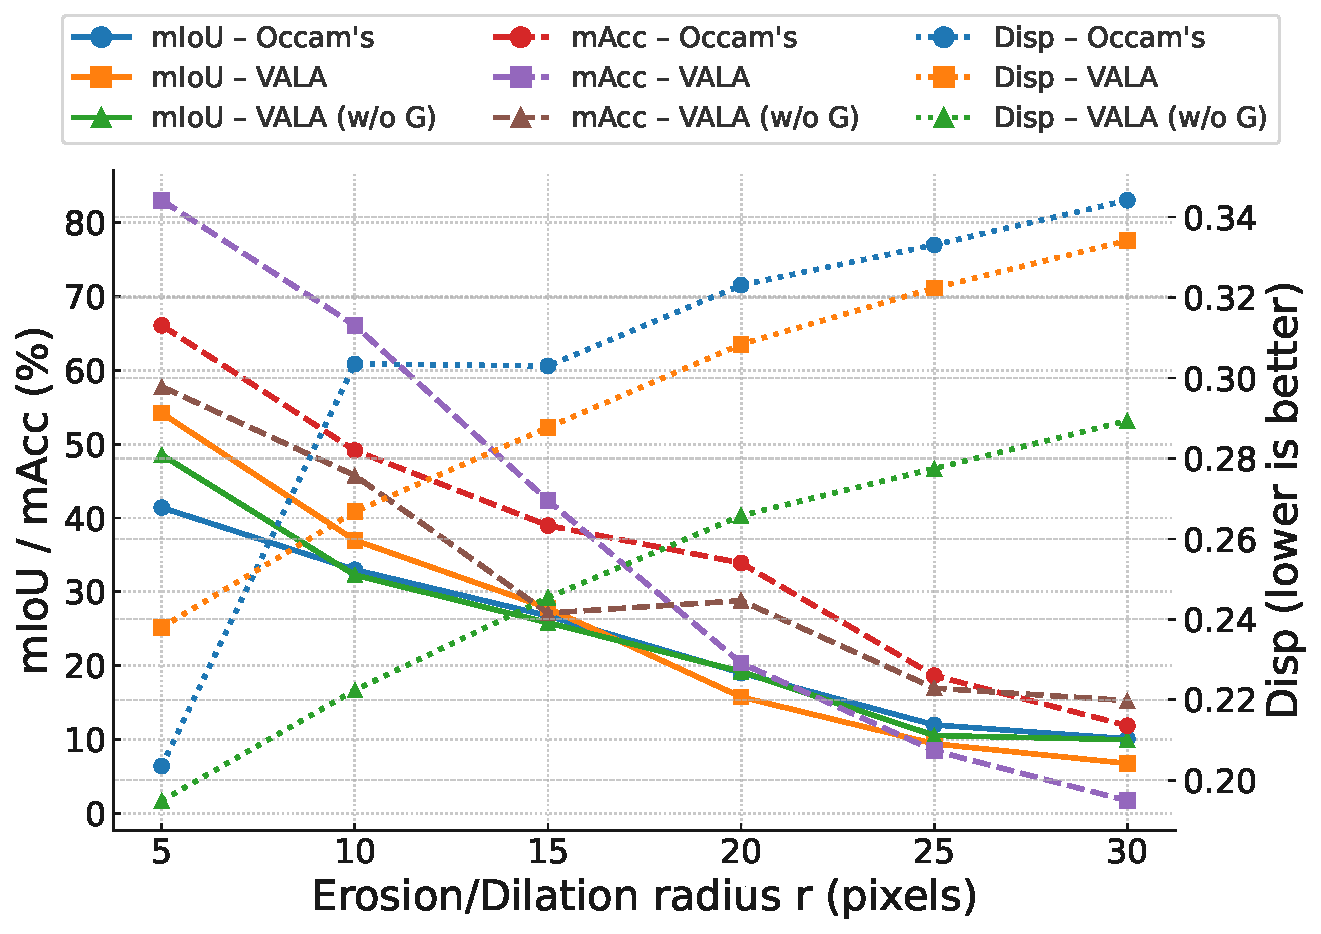
\includegraphics[width=0.95\linewidth]{supp_figs/vala_stress_test_curve_legend_top_halfdown.pdf} % png/jpg/pdf 都行
  \caption{Robustness under mask boundary corruptions. mIoU/mAcc (\%) are shown on the left $y$-axis; \textit{Disp} (lower is better) on the right $y$-axis. 
  We vary the erosion/dilation radius $r$ (pixels). 
  VALA degrades more slowly than Occam’s and its ablation without gating (VALA w/o G), while achieving lower \textit{Disp} across severities.}
  \label{fig:robustness}
\end{figure}


To evaluate robustness against segmentation noise, we perform an experiment on the teatime scene of LERF-OVS by simulating errors in SAM masks.

\textbf{Stress-Testing Robustness with Corrupted Masks.}
To stress-test robustness against imperfect proposals, 
we corrupt each SAM mask by a per-mask morphological perturbation applied at the original image resolution. 
Let $m_k \in \{0,1\}^{H\times W}$ denote the binary mask of instance $k$, 
and let
\[
B_r = \{(x,y)\in\mathbb{Z}^2 : x^2 + y^2 \leq r\}
\]
be a disk-shaped structuring element of radius $r$ pixels, where $r \in {5,10,15,20,25,30}$, to simulate different perturbation levels.

For every mask we draw an independent sign variable $\sigma_k \in \{-1,+1\}$ with equal probability 
$P(\sigma_k=+1)=P(\sigma_k=-1)=0.5$. 
The corrupted mask $\tilde{m}_k$ is then
\[
\tilde{m}_k =
\begin{cases}
m_k \,\ominus\, B_r, & \text{if } \sigma_k=-1 \quad \text{(erosion)}, \\[4pt]
m_k \,\oplus\, B_r, & \text{if } \sigma_k=+1 \quad \text{(dilation)},
\end{cases}
\]
where $\ominus$ and $\oplus$ denote morphological erosion and dilation, respectively.  

To prevent degenerate outcomes on small objects, we enforce a non-vanishing guard: 
if erosion yields an empty or tiny region (area below a minimum threshold $\tau_{\min}$ pixels), 
we fallback to dilation and set $\tilde{m}_k \leftarrow m_k \oplus B_r$.  
After corruption, we recompute tight bounding boxes from $\tilde{m}_k$ 
and propagate them to downstream steps (e.g., cropping and $224\times224$ resizing for CLIP feature extraction).  

This perturbation stochastically shifts boundaries outward/inward by approximately $r$ pixels 
while preserving instance identity, thereby simulating over- and under-segmentation errors 
commonly observed in practice.

\begin{figure*}[t]
    \centering
    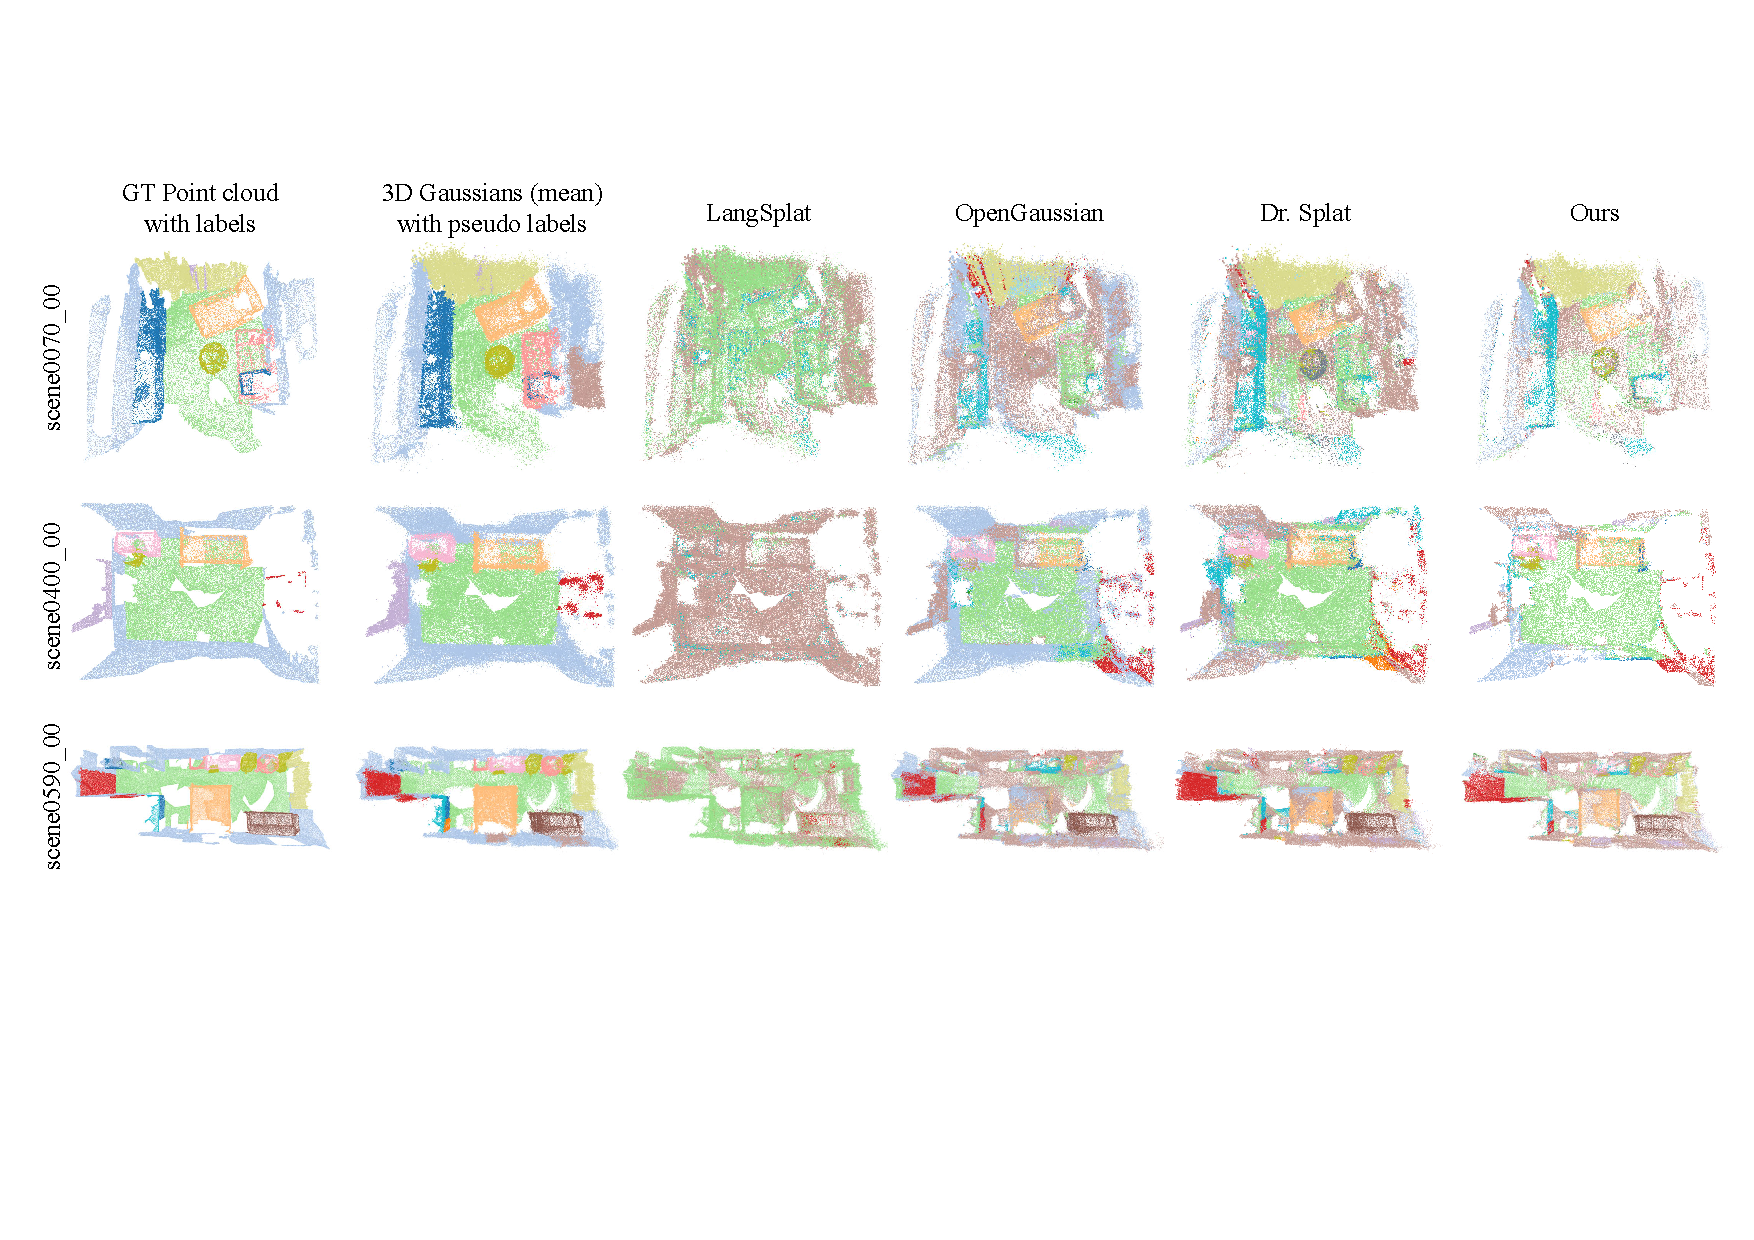
\includegraphics[width=\textwidth]{supp_figs/supp_qualitative_scannet.pdf}
    \caption{More qualitative results of 3D semantic segmentation on the ScanNet-v2 dataset~\cite{dai2017scannet},}
    \label{fig:more_qualitative_scannet}
\end{figure*}

\textbf{Evaluation Protocal.}
To assess the robustness of the proposed streaming median in the cosine space, we compare three variants: the baseline Occam's LGS~\cite{cheng2024occam}, our full model incorporating both visibility-aware gating and robust multi-view aggregation (VALA), and an ablation variant with only the robust multi-view aggregation module (VALA w/o G). In addition to the standard mIoU and mAcc metrics for evaluating the final 3D object selection task, we further introduce the \emph{dispersion} score, which specifically quantifies the robustness of assigned language features under multi-view variations.
Given a Gaussian $g_i$ with observed unit features $f_{i}^s \in \mathbb{S}^{d-1}$, the per-Gaussian dispersion is computed as
\begin{equation}
\mathrm{Disp}_i = \frac{1}{|S_i|}\sum_{(i,s)\in S_i}\Big(1-\langle f_i^s, z_i^*\rangle\Big),
\end{equation}

\noindent
At the scene level, we report the average:

\begin{equation}
\mathrm{Disp}_{\text{scene}} = \frac{1}{|I|}\sum_{i\in I}\mathrm{Disp}_i,
\end{equation}

\noindent
This metric captures the average misalignment between observed features and the aggregated Gaussian feature, where lower values indicate higher consistency.

\begin{figure*}[t]
    \centering
    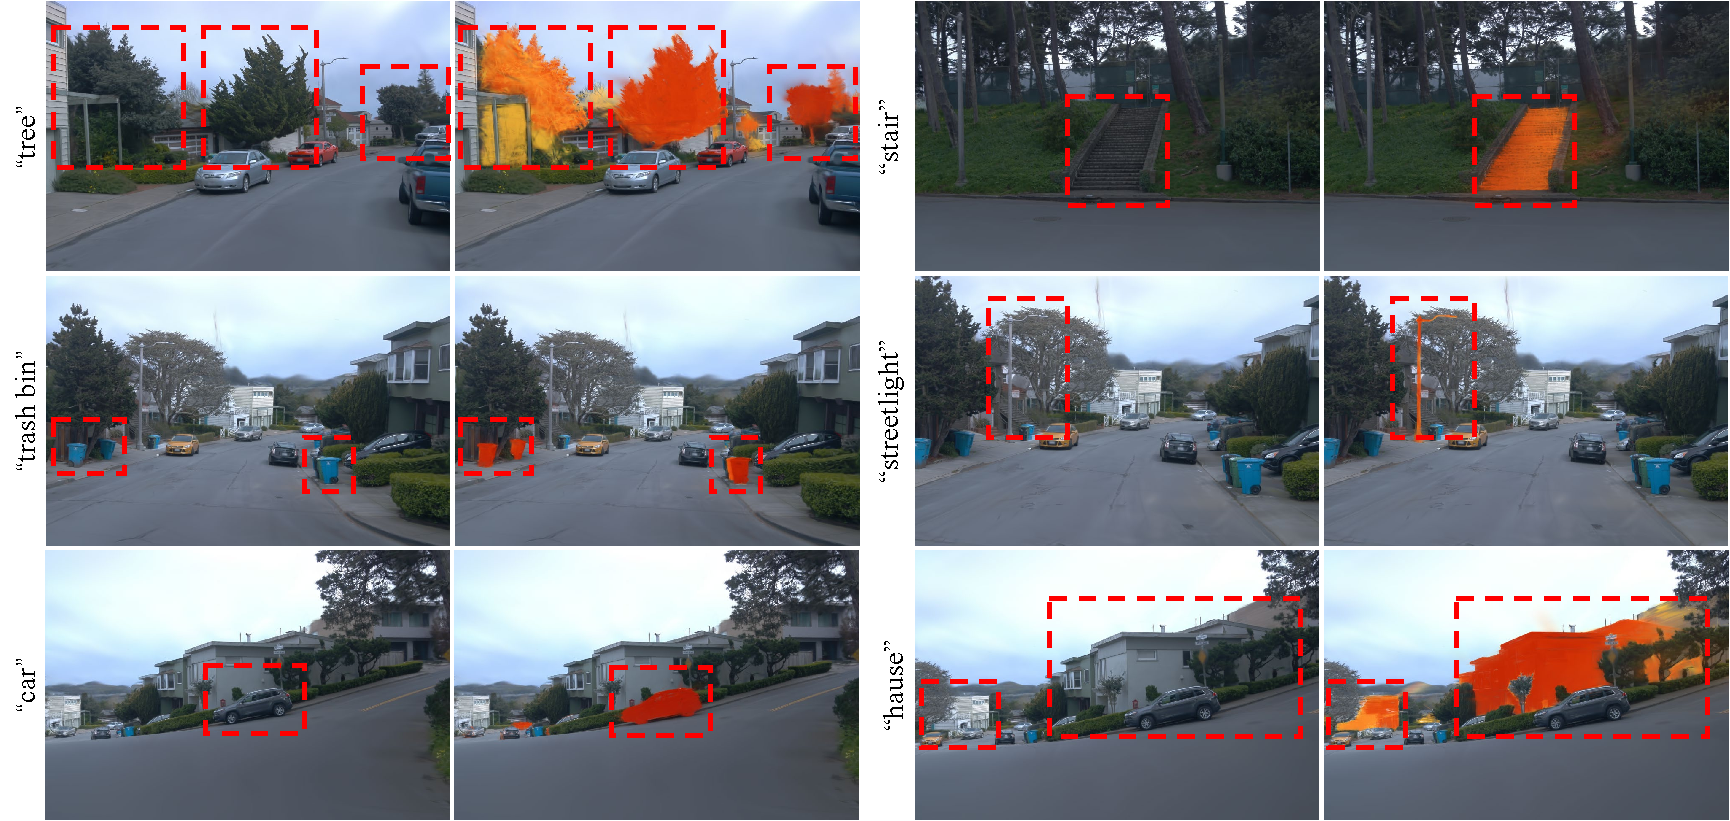
\includegraphics[width=\textwidth]{supp_figs/qualitative_waymo.pdf}
    \caption{\textbf{Qualitative results on the Waymo Open Dataset~\cite{Sun_2020_CVPR}}. The colored regions indicate the activation maps corresponding to the given text prompts.}
    \label{fig:quantitative_waymo}
\end{figure*}
    

\textbf{Results Analysis.}
The results are presented in \figureautorefname~\ref{fig:robustness}. As the corruption radius increases from $r=5$ to $30$ px, all methods show a monotonic decline in mIoU/mAcc and a corresponding rise in Disp, confirming that boundary noise simultaneously degrades semantic accuracy and cross-view consistency. Importantly, the deterioration is substantially slower for our methods than for Occam’s LGS, as reflected by the smaller slope of Disp. In terms of accuracy, VALA achieves the strongest results: at $r=5$, it surpasses Occam’s by +12.8 mIoU and +17.0 mAcc, with substantial gains still observed at $r=10$. Meanwhile, the Disp values reveal a complementary trend—although VALA’s Disp is marginally higher than Occam’s at $r=5$, it drops below Occam’s from $r=10$ onwards. This demonstrates that the combination of visibility-aware gating and robust aggregation not only improves accuracy but also enhances multi-view consistency in the practically relevant regime of mild mask noise.

When boundary damage becomes severe, however, the picture changes. VALA (w/o G) overtakes the full VALA model in accuracy (e.g., at $r=30$, achieving 9.95/15.25 vs.\ 6.75/1.69 in mIoU/mAcc) and consistently yields the lowest Disp across all radii. This suggests that the fixed gating threshold becomes overly conservative under extreme corruption, discarding too many observations and leaving insufficient evidence for many Gaussians. In contrast, the cosine-median aggregator alone remains robust, preserving both accuracy and consistency in this challenging setting. Overall, these results highlight a clear regime split: visibility-aware gating combined with a cosine median provides the strongest accuracy and consistency under realistic (mild to moderate) noise. However, under extreme boundary corruption, robust aggregation is the key factor, as overly strict gating thresholds reduce coverage and performance.

\section{Additional Results}
\label{subsec:add_results}
In this section, we present additional results on the ScanNet dataset and, more importantly, demonstrate that our algorithm can be applied to real-world outdoor datasets, achieving superior open-vocabulary semantic segmentation in autonomous driving scenarios.

\textbf{More Qualitative Results on the ScanNet Dataset.}
We provide additional qualitative results on three bedrooms with varying levels of complexity and clutter. Across all scenes, competing methods struggle to correctly recognize the bed (highlighted in orange); the occluded portions near the wall are consistently misclassified as adjacent categories, such as the wall or floor. This issue persists in the third scene, where the bed is fragmented into multiple categories. In contrast, our method preserves the bed as a coherent instance, owing to the proposed gating module that explicitly handles low-visibility Gaussians.

\textbf{Experiments on the Waymo Open Dataset.} To further validate our algorithm’s generalization capability in real-world outdoor environments, we conduct experiments on the Waymo Open Dataset~\cite{Sun_2020_CVPR}. This dataset is a large-scale, high-quality autonomous driving benchmark that provides synchronized LiDAR and multi-camera data collected across diverse urban and suburban geographies, along with comprehensive 2D/3D annotations and tracking identifiers.
For evaluation, we select a sequence captured in a residential neighborhood that contains rich semantic elements, such as vehicles, vegetation, street infrastructure, and buildings. We focus on five of the most common outdoor categories, e.g. \textit{tree}, \textit{trash bin}, \textit{car}, \textit{streetlight}, and \textit{house}, as well as one tail category, \textit{stair}. The qualitative results in \figureautorefname~\ref{fig:quantitative_waymo} demonstrate that our method achieves precise open-vocabulary 3D semantic segmentation on outdoor data. Both small-scale objects (e.g., trash bins and streetlights) and large-scale objects (e.g., trees, cars, and houses) are not only correctly retrieved but also segmented with sharp boundaries, reflecting the accurate registration of language features on the 3D Gaussian Splatting representation. Notably, our method remains robust under occlusion owing to the proposed visibility-aware gating module. For example, correctly delineating trees behind metallic structures or houses partially obscured by vegetation.

These findings emphasize the robustness and versatility of our method when transferred from indoor (ScanNet) to challenging outdoor driving scenarios, underscoring its strong potential for real-world autonomous driving applications. A supplementary video is included to further demonstrate the effectiveness and the multi-view consistency of our method. 

\section{Limitations}
\label{subsec:limt}

While our approach demonstrates strong performance across multiple tasks, including 2D and 3D object selection as well as 3D semantic segmentation, and exhibits notable generalization to cross-domain settings such as outdoor datasets, certain limitations remain. To assess robustness against noisy SAM masks, we conducted stress tests with multi-scale morphological perturbations. The results show that our visibility-aware gating achieves superior mIoU and mAcc under moderate noise, while the proposed cosine median maintains low dispersion even under severe corruption, indicating the effectiveness of our robust feature aggregator. However, our current framework relies on a fixed threshold to prune Gaussians, which can become overly conservative under extreme noise, resulting in degraded multi-view consistency. Moreover, our method is specifically designed for static scenes and does not naturally extend to dynamic environments. Future work will therefore focus on developing adaptive, scene-aware thresholds and extending our framework to handle dynamic scenes.
